% An evenly covered open set U: its preimage is a stack of disjoint sheets, each
% mapped homeomorphically onto U by p.
% Source: book/tex/topology/cover-project.tex (§ Even coverings and covering projections).
\documentclass[border=2mm]{standalone}
\usepackage{tikz}
\usepackage{amssymb}
\usetikzlibrary{arrows.meta,decorations.pathreplacing}
\begin{document}
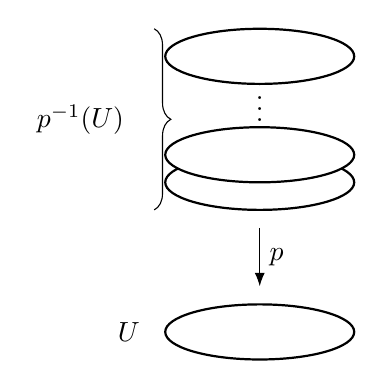
\begin{tikzpicture}[scale=1]
  % the sheets over U
  \draw[thick,fill=white] (0,3.2) ellipse (1.2 and 0.35);
  \node at (0,2.64) {$\vdots$};
  \draw[thick,fill=white] (0,1.6) ellipse (1.2 and 0.35);
  \draw[thick,fill=white] (0,1.95) ellipse (1.2 and 0.35);
  % brace labelling the preimage
  \draw[decorate,decoration={brace,amplitude=6pt}] (-1.34,3.55) -- (-1.34,1.25);
  \node[left] at (-1.6,2.4) {$p^{-1}(U)$};
  % projection
  \draw[-{Latex}] (0,1.02) -- (0,0.28) node[midway,right] {$p$};
  % U itself
  \draw[thick] (0,-0.3) ellipse (1.2 and 0.35);
  \node[left] at (-1.4,-0.3) {$U$};
\end{tikzpicture}
\end{document}
